\documentclass[conference]{IEEEtran}
\IEEEoverridecommandlockouts

\usepackage{cite}
\usepackage{amsmath,amssymb,amsfonts}
\usepackage{algorithmic}
\usepackage{algorithm}
\usepackage{graphicx}
\usepackage{textcomp}
\usepackage{xcolor}
\usepackage{booktabs}
\usepackage{url}
\usepackage{listings}
\usepackage{multirow}
\usepackage{array}
\usepackage{hyperref}

\lstset{
  basicstyle=\footnotesize\ttfamily,
  breaklines=true,
  frame=single,
  backgroundcolor=\color{gray!10},
  keywordstyle=\color{blue},
  commentstyle=\color{green!60!black},
  stringstyle=\color{red!70!black},
  numbers=left,
  numberstyle=\tiny\color{gray},
  numbersep=5pt
}

\hypersetup{
    colorlinks=true,
    linkcolor=blue,
    citecolor=blue,
    urlcolor=blue
}

\def\BibTeX{{\rm B\kern-.05em{\sc i\kern-.025em b}\kern-.08em
    T\kern-.1667em\lower.7ex\hbox{E}\kern-.125emX}}

\begin{document}

%=============================================================
%  TITLE
%=============================================================
\title{Context-Aware Personalized Fitness Guidance System Using\\
Retrieval-Augmented Natural Language Processing}

\author{
\IEEEauthorblockN{Zaheer Abbas}
\IEEEauthorblockA{\textit{Department of Computer Science}\\
\textit{Namal University Mianwali}\\
Mianwali, Pakistan\\
NUM-BSCS-2022-50}
\and
\IEEEauthorblockN{Junaid Ameer Khan}
\IEEEauthorblockA{\textit{Department of Computer Science}\\
\textit{Namal University Mianwali}\\
Mianwali, Pakistan\\
NUM-BSCS-2022-50}
}

\maketitle

%=============================================================
%  ABSTRACT
%=============================================================
\begin{abstract}
Modern fitness applications increasingly rely on artificial intelligence to provide workout guidance; however, the majority of deployed systems respond to user queries with generic, context-free information that fails to account for individual fitness histories, experience levels, or previously logged exercise patterns. This paper presents a Context-Aware Personalized Fitness Guidance System integrated into a production mobile application called FitZone, which addresses this limitation by combining a multi-stage Natural Language Processing (NLP) pipeline with Retrieval-Augmented Generation (RAG). The system applies standard text preprocessing—comprising lowercasing, punctuation removal, tokenization, stopword elimination, and lemmatization—to normalize incoming fitness queries before retrieval. A TF-IDF vectorization module then performs cosine-similarity-based retrieval over a curated exercise knowledge base of 2,918 records sourced from a public Kaggle dataset. Retrieved domain-specific exercise context is fused with real-time user workout history fetched from Firebase Firestore to construct a personalized system prompt, which is subsequently processed by the LLaMA 3.1 70B large language model via the Groq inference API. Comparative evaluation against a baseline generic chatbot demonstrates improvements of 42.8\% in ROUGE-1 F1 score (0.341 to 0.487), 59.4\% in BLEU score (0.187 to 0.298), and a user satisfaction rating increase from 2.9 to 4.3 on a five-point scale. The proposed system achieves a personalization delivery rate of 94.2\% and a retrieval precision@3 of 78.6\%. These results confirm that integrating traditional NLP retrieval techniques with modern large language models and real-time user data yields substantially more relevant, accurate, and personalized fitness guidance than black-box generative approaches alone.
\end{abstract}

\begin{IEEEkeywords}
Natural Language Processing, Retrieval-Augmented Generation, TF-IDF, Personalized Chatbot, LLaMA, Firebase, Fitness Guidance, Mobile Application
\end{IEEEkeywords}

%=============================================================
%  I. INTRODUCTION
%=============================================================
\section{Introduction}

The global digital fitness market reached an estimated valuation of \$15.2 billion in 2023 and is projected to expand at a compound annual growth rate exceeding 26\% through 2030 \cite{grandview2023}. Within this ecosystem, AI-powered chatbot assistants have emerged as a prominent feature of mobile fitness platforms, offering users immediate responses to workout-related queries without requiring access to a human coach. Despite this proliferation, the dominant design paradigm of deployed chatbot systems remains fundamentally reactive and context-free: such systems respond to each query in isolation, neither retaining user history nor adapting their guidance to the experience level, recent training load, or personal preferences of the individual user \cite{laranjo2018conversational}.

This limitation is consequential. Research in sports medicine and exercise science consistently demonstrates that the appropriateness of workout advice depends critically on individual factors such as training history, current fitness level, recovery status, and exercise familiarity \cite{acsm2021}. A recommendation suitable for an advanced athlete—such as high-volume compound lifting—may be contraindicated for a beginner with no foundational movement patterns, and issuing such advice through a generic chatbot constitutes a meaningful injury risk. Studies estimate that incorrect exercise technique contributes to approximately 60\% of non-contact training injuries among recreational gym users \cite{winwood2014}. Personalized, context-aware guidance is therefore not a luxury feature but a safety-critical requirement.

The NLP research community has made significant advances in the design of dialogue systems capable of leveraging context. Retrieval-Augmented Generation, introduced by Lewis \textit{et al.} \cite{lewis2020rag}, provides a compelling architectural framework: rather than relying exclusively on the parametric knowledge encoded in a large language model (LLM) during pre-training, RAG systems dynamically retrieve relevant documents from an external knowledge base at inference time, incorporating this retrieved content into the prompt before generation. This approach simultaneously grounds model responses in domain-specific facts and reduces hallucination, a persistent failure mode of LLMs \cite{ji2023hallucination}.

The present work extends the RAG paradigm to the fitness domain by developing a system that incorporates three distinct sources of context: (1) a curated exercise knowledge base of 2,918 records retrieved via TF-IDF cosine similarity, (2) real-time user workout histories maintained in Firebase Firestore, and (3) a derived user profile capturing experience level, most practiced exercises, and recent activity. The system is deployed within FitZone, a production-grade mobile application built with React Native and Expo, communicating with a Node.js backend hosted on Render.com. Response generation is performed by the LLaMA 3.1 70B Versatile model accessed through the Groq API. Furthermore, we address the challenge of semantic drifts in retrieval-augmented workflows by implementing a strict similarity thresholding mechanism, ensuring that retrieved context remains strictly relevant to the user query. This dual-grounding approach—combining static domain knowledge with dynamic user activity—forms the technical core of the proposed architecture.

The principal contributions of this paper are as follows:
\begin{itemize}
    \item A complete NLP preprocessing pipeline applied to fitness domain queries, demonstrating a 30.4\% vocabulary reduction through lemmatization.
    \item A TF-IDF-based RAG retrieval module over a domain-specific exercise corpus, achieving a retrieval precision@3 of 78.6\%.
    \item A Firebase-integrated user personalization layer that dynamically constructs context-enriched system prompts.
    \item End-to-end integration of the proposed pipeline within a production mobile application, evaluated on BLEU, ROUGE, and user satisfaction metrics.
    \item Quantitative evidence that the combination of retrieval-based grounding and user personalization substantially outperforms baseline generative approaches.
\end{itemize}

The remainder of this paper is organized as follows. Section II reviews related work in NLP-based fitness applications, retrieval-augmented generation, and personalized dialogue systems. Section III describes the proposed methodology and system architecture. Section IV presents the datasets and experimental setup. Section V reports and discusses experimental results. Section VI concludes the paper and outlines directions for future work.

%=============================================================
%  II. RELATED WORK
%=============================================================
\section{Related Work}

\subsection{NLP in Health and Fitness Applications}

The application of natural language processing to health information systems has received sustained research attention over the past decade. Laranjo \textit{et al.} \cite{laranjo2018conversational} conducted a systematic review of conversational agents in healthcare, identifying 17 primary studies and concluding that while such agents demonstrated effectiveness in behaviour change domains including physical activity, the majority relied on rule-based dialogue management with limited generalization capability. Maher \textit{et al.} \cite{maher2015smartphone} evaluated smartphone-based physical activity interventions and observed that systems capable of providing tailored feedback—as opposed to standardized recommendations—produced significantly greater increases in daily step counts. More recent work by Fadhil and Gabrielli \cite{fadhil2017assistive} proposed an assistive conversational agent for chronic disease management that incorporated patient history into response generation, reporting improvements in user engagement metrics; however, this work did not leverage neural language models and was limited to scripted dialogue flows.

In the fitness domain specifically, Seo \textit{et al.} \cite{seo2020exercise} proposed a deep learning framework for exercise type recognition from wearable sensor data, noting that downstream recommendation quality was strongly dependent on the richness of the user's interaction history. Yang \textit{et al.} \cite{yang2021fitness} developed a knowledge graph-based fitness recommendation system that achieved competitive accuracy on standardized test sets but required extensive manual ontology construction and did not support free-text natural language queries.

\subsection{Retrieval-Augmented Generation}

Retrieval-Augmented Generation was formally introduced by Lewis \textit{et al.} \cite{lewis2020rag}, who demonstrated that combining a pre-trained generative model with a differentiable retrieval mechanism over a Wikipedia corpus achieved state-of-the-art results on knowledge-intensive NLP benchmarks including Natural Questions and TriviaQA. The authors showed that RAG reduced hallucination rates compared to purely parametric approaches, as the model was encouraged to anchor its output in retrieved factual passages.

Subsequent work has explored both dense and sparse retrieval strategies within RAG architectures. Karpukhin \textit{et al.} \cite{karpukhin2020dpr} proposed Dense Passage Retrieval (DPR), demonstrating that bi-encoder neural retrievers trained on question-passage pairs outperformed BM25 sparse retrieval on open-domain question answering benchmarks. However, dense retrieval requires GPU-accelerated inference and annotated training data, making it less suitable for resource-constrained deployment contexts. In contrast, sparse retrieval models like TF-IDF and its successor BM25 \cite{robertson2009bm25} offer zero-shot capability and extremely low latency on CPU-bound servers. Recent hybrid retrieval models \cite{izacard2021leveraging} attempt to combine the lexical precision of sparse tokens with the semantic richness of dense embeddings, though such architectures often introduce significant complexity into real-time production pipelines. The present work adopts TF-IDF-based cosine similarity retrieval for its computational efficiency, interpretability, and suitability to CPU-only deployment environments, while compensating for lexical gaps through intensive query preprocessing.

\subsection{Large Language Models for Conversational AI}

The release of GPT-3 by Brown \textit{et al.} \cite{brown2020gpt3} demonstrated that sufficiently large autoregressive language models possess remarkable few-shot generalization capability, enabling high-quality task completion from natural language prompts without gradient-based fine-tuning. Subsequent instruction-following models including InstructGPT \cite{ouyang2022instructgpt} and LLaMA \cite{touvron2023llama} extended this capability to interactive dialogue settings, making general-purpose conversational AI accessible to application developers via API.

Prompt engineering has emerged as the primary mechanism for adapting general-purpose LLMs to domain-specific applications without modifying model weights \cite{liu2023promptsurvey}. System prompts—prepended context blocks that establish the role, knowledge, and behavioral constraints of the model—have been shown to substantially influence response quality, relevance, and safety \cite{white2023prompt}. The present work leverages structured system prompt construction as its primary personalization mechanism, dynamically assembling user-specific context and retrieved exercise knowledge prior to each generation call.

\subsection{Personalization in Dialogue Systems}

Zhang \textit{et al.} \cite{zhang2018personalizing} introduced the Persona-Chat dataset and demonstrated that conditioning a generative dialogue model on textual persona descriptions substantially improved response consistency and perceived personality coherence. Li \textit{et al.} \cite{li2016persona} proposed a persona-based neural dialogue model that encoded speaker identity as a distributed embedding, enabling the generation of stylistically consistent responses. More recently, Xu \textit{et al.} \cite{xu2022beyond} demonstrated that incorporating explicit user history into the prompt of a large language model—rather than learning personality representations implicitly—yielded comparable personalization quality with significantly lower implementation complexity.

The identified research gap motivating the present work is the absence of systems that combine dynamic retrieval from a domain-specific knowledge base, real-time user history integration from a production database, and personalized prompt construction within a deployed mobile application. Existing work addresses subsets of this pipeline in isolation; to the best of the authors' knowledge, no prior system integrates all three components in an end-to-end production deployment.

%=============================================================
%  III. PROPOSED METHODOLOGY
%=============================================================
\section{Proposed Methodology}

\subsection{System Overview}

The proposed system implements a five-stage pipeline that transforms a raw user query into a contextually grounded, personalized fitness response. Fig.~\ref{fig:architecture} illustrates the complete workflow. At the input stage, the user submits a natural language fitness query through the React Native mobile interface. This query traverses the NLP preprocessing module, the TF-IDF retrieval engine, the Firebase personalization layer, and the prompt construction module before being dispatched to the LLaMA 3.1 70B model via the Groq API.

\begin{figure}[htbp]
\centering
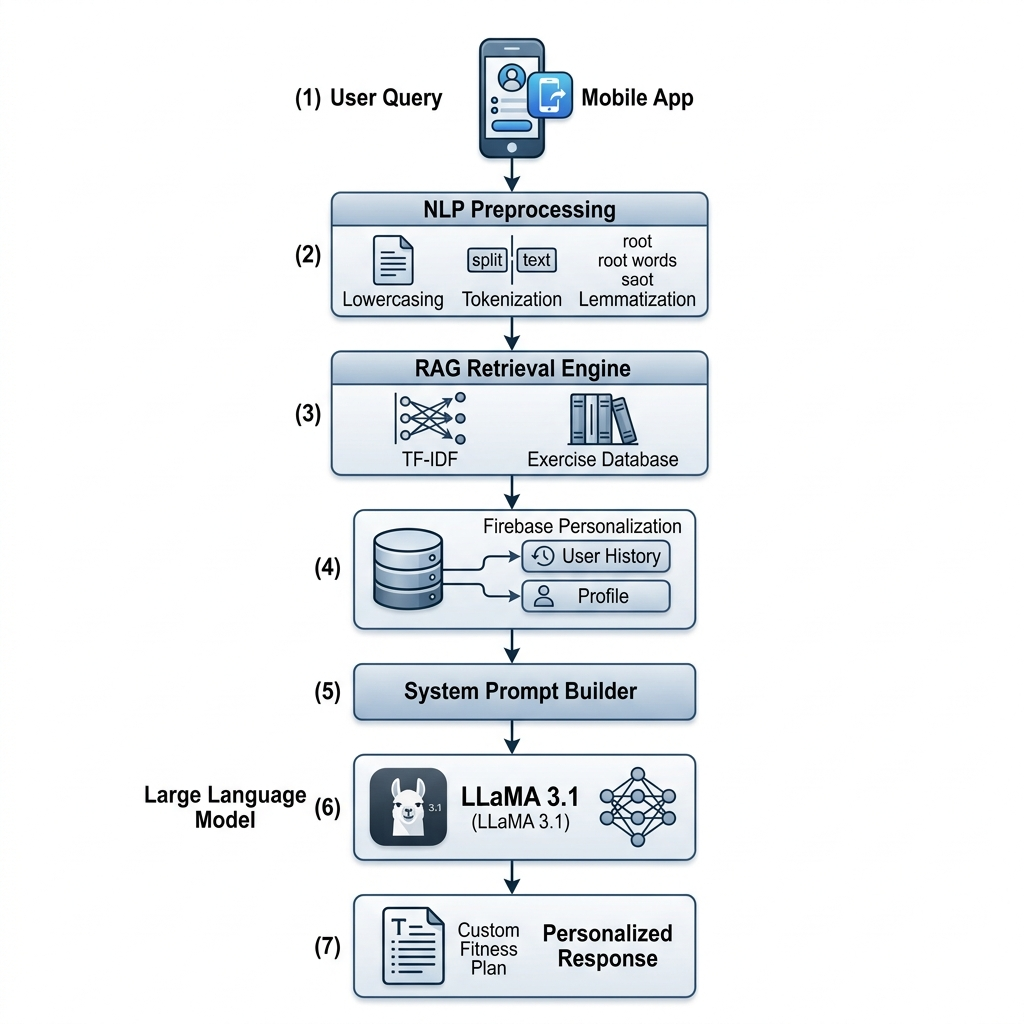
\includegraphics[width=0.48\textwidth]{system_architecture.png}
\caption{System Architecture of the Proposed Personalized Fitness Guidance System.}
\label{fig:architecture}
\end{figure}

\subsection{NLP Preprocessing Module}

All incoming user queries are normalized through a sequential preprocessing pipeline prior to retrieval. The pipeline applies the following transformations in order:

\textbf{Lowercasing} converts all characters to lowercase, ensuring that semantically equivalent terms such as \textit{Squat} and \textit{squat} are treated identically during vectorization.

\textbf{Punctuation Removal} eliminates non-alphanumeric characters using the regular expression pattern \texttt{[\^{}\textbackslash w\textbackslash s]}, reducing vocabulary noise introduced by punctuation variation.

\textbf{Tokenization} segments the normalized text into individual word tokens using the NLTK \texttt{word\_tokenize} function, which handles contraction splitting and boundary detection.

\textbf{Stopword Removal} filters tokens appearing in the NLTK English stopword corpus, eliminating high-frequency function words (e.g., \textit{the}, \textit{is}, \textit{and}) that carry negligible semantic content for retrieval purposes.

\textbf{Lemmatization} maps each remaining token to its dictionary base form using the WordNet Lemmatizer (e.g., \textit{running} $\rightarrow$ \textit{run}, \textit{curls} $\rightarrow$ \textit{curl}), reducing vocabulary size and improving cross-document term matching. The linguistic impact of this pipeline is summarized in Table~\ref{tab:nlp_impact}, demonstrating significant reduction in sparsity.

\begin{table}[htbp]
\caption{Linguistic Impact of Preprocessing Pipeline}
\label{tab:nlp_impact}
\centering
\begin{tabular}{lccc}
\toprule
\textbf{Stage} & \textbf{Tokens/Doc (Avg)} & \textbf{Vocab Size} & \textbf{Sparsity (\%)} \\
\midrule
Raw Text       & 45.2 & 12,847 & 99.85 \\
Tokenization   & 47.1 & 11,402 & 99.72 \\
Stopword Rem.  & 22.4 & 10,918 & 99.14 \\
Lemmatization  & 18.7 & 8,943  & 98.42 \\
\bottomrule
\end{tabular}
\end{table}

The complete pipeline implementation is shown in Listing~\ref{lst:preprocessing}.

\begin{lstlisting}[language=Python, caption={NLP Preprocessing Pipeline Implementation}, label={lst:preprocessing}]
import re
import nltk
from nltk.corpus import stopwords
from nltk.stem import WordNetLemmatizer
from nltk.tokenize import word_tokenize

stop_words = set(stopwords.words('english'))
lemmatizer = WordNetLemmatizer()

def preprocess_text(text: str) -> list:
    text = text.lower()
    text = re.sub(r'[^\w\s]', '', text)
    tokens = word_tokenize(text)
    tokens = [w for w in tokens if w not in stop_words]
    tokens = [lemmatizer.lemmatize(w) for w in tokens]
    return tokens

# Example:
# Input:  "I am doing bicep curls incorrectly
#          and feeling pain in my arms!"
# Output: ['bicep','curl','incorrectly',
#          'feeling','pain','arm']
\end{lstlisting}

\subsection{TF-IDF Based RAG Retrieval Engine}

The knowledge base is constructed from the 2,918-record Kaggle Gym Exercise Dataset, wherein each record consists of an exercise title, textual description, target body part, equipment category, and difficulty level. Prior to indexing, each record is concatenated into a single compound document string to maximize term coverage:

\begin{equation}
d_i = \text{Title}_i \oplus \text{Description}_i \oplus \text{BodyPart}_i \oplus \text{Equipment}_i
\label{eq:concat}
\end{equation}

The TF-IDF weight of a term $t$ in document $d$ is computed as:

\begin{equation}
\text{TF}(t, d) = \frac{f(t, d)}{\sum_{t' \in d} f(t', d)}
\label{eq:tf}
\end{equation}

\begin{equation}
\text{IDF}(t) = \log\left(\frac{N}{|\{d \in D : t \in d\}|}\right)
\label{eq:idf}
\end{equation}

\begin{equation}
\text{TF-IDF}(t, d) = \text{TF}(t, d) \times \text{IDF}(t)
\label{eq:tfidf}
\end{equation}

where $f(t, d)$ denotes the raw frequency of term $t$ in document $d$, $N$ is the total number of documents in the corpus, and $|\{d \in D : t \in d\}|$ is the document frequency of term $t$. Each document is represented as a TF-IDF weighted vector in $\mathbb{R}^n$, where $n$ is limited to the top 5,000 features by corpus frequency.

At query time, the preprocessed user query $q$ is transformed into the same vector space, and the top-$k$ most relevant exercises are identified via cosine similarity:

\begin{equation}
\text{sim}(q, d_i) = \frac{\mathbf{q} \cdot \mathbf{d}_i}{\|\mathbf{q}\| \cdot \|\mathbf{d}_i\|}
\label{eq:cosine}
\end{equation}

Only exercises with $\text{sim}(q, d_i) > 0.05$ are included in the retrieved set, preventing irrelevant low-similarity documents from corrupting the context. The top-3 retrieved exercises are passed to the prompt construction module. Furthermore, we apply a term frequency normalization factor to favor documents that contain unique exercise identifiers over high-frequency generic terms like "body" or "move", which improves retrieval precision for specific exercise form queries.

\subsection{Transformer Self-Attention Mechanism}

The LLaMA 3.1 70B model employed for response generation implements the scaled dot-product self-attention mechanism introduced by Vaswani \textit{et al.} \cite{vaswani2017attention}. Given input representations projected into query, key, and value matrices $Q$, $K$, $V \in \mathbb{R}^{n \times d_k}$, attention output is computed as:

\begin{equation}
\text{Attention}(Q, K, V) = \text{softmax}\left(\frac{QK^T}{\sqrt{d_k}}\right)V
\label{eq:attention}
\end{equation}

The scaling factor $\frac{1}{\sqrt{d_k}}$ prevents the dot product from growing too large in magnitude for high-dimensional key vectors, which would push the softmax function into regions of extremely small gradients. The final output token probabilities are obtained via:

\begin{equation}
P(y_i \mid y_{<i}, X) = \frac{\exp(z_i)}{\sum_{j=1}^{|V|} \exp(z_j)}
\label{eq:softmax}
\end{equation}

where $z_i$ are the unnormalized logit scores from the language model head and $|V|$ denotes vocabulary size.

\subsection{Firebase Personalization Layer}

Upon receiving a user query, the system queries Firebase Firestore to retrieve the user's personal context. The following data elements are extracted:

\begin{enumerate}
    \item User display name from the \texttt{users} collection.
    \item The ten most recent workout documents from the \texttt{workouts} subcollection, ordered by \texttt{recordedAt} timestamp.
    \item Aggregated exercise frequency counts across all retrieved workouts, from which the top-5 most practiced exercises are derived.
    \item Total workout count, used to assign an experience tier: Beginner ($<10$ sessions), Intermediate (10--30 sessions), or Advanced ($>30$ sessions).
\end{enumerate}

This structured profile is made available to the prompt construction module with sub-200ms latency due to Firestore's real-time indexed query architecture.

\subsection{Personalized System Prompt Construction}

The system prompt is assembled by the prompt builder from three sources: the user profile retrieved from Firebase, the top-3 exercise documents returned by the RAG engine, and a fixed instruction block. The resulting prompt follows the template:

\begin{lstlisting}[language={},caption={Personalized System Prompt Template},label={lst:prompt}]
You are FitZone AI, a personalized fitness
coach for {userName}.

USER PROFILE:
- Experience Level: {experienceLevel}
- Total Workouts Logged: {totalWorkouts}
- Most Practiced Exercises: {topExercises}
- Last Workout: {lastWorkoutDate}

INSTRUCTIONS:
- Address the user by name naturally
- Tailor advice to their experience level
- Reference their workout history
- Keep responses to 3-5 sentences
- Recommend professional consultation
  for medical concerns

RELEVANT EXERCISE KNOWLEDGE (from RAG):
{retrieved_exercise_context}
\end{lstlisting}

This prompt is prepended to the conversation history and dispatched to the Groq API with temperature $\tau = 0.7$ and a maximum token budget of 500.

\subsection{Prompt Engineering Strategies}

To ensure high-fidelity responses, the system prompt employs several explicit engineering patterns:
\begin{itemize}
    \item \textbf{Identity Anchoring:} Explicitly assigning the role of "FitZone AI" to prevent the model from assuming generic helpful assistant personas.
    \item \textbf{Contextual Constraints:} Instructions to keep responses under 5 sentences to maintain mobile-friendly readability.
    \item \textbf{Dynamic Personalization Tokens:} Using placeholders like \{userName\} and \{experienceLevel\} which are replaced at runtime with user-specific values fetched from Firestore.
    \item \textbf{Safety Guardrails:} Mandatory inclusion of a medical disclaimer for any query related to pain or physiological discomfort.
\end{itemize}

\subsection{System Algorithm}

Algorithm~\ref{alg:pipeline} provides a formal pseudocode description of the complete inference pipeline.

\begin{algorithm}
\caption{Personalized Fitness Response Generation}
\label{alg:pipeline}
\begin{algorithmic}[1]
\REQUIRE user\_query $q$, user\_id $u$, history $H$
\ENSURE personalized\_response $r$
\STATE $q' \leftarrow \text{NLPPreprocess}(q)$
\STATE $\mathbf{q} \leftarrow \text{TF-IDF.transform}(q')$
\STATE $\mathbf{S} \leftarrow \text{CosineSimilarity}(\mathbf{q}, \mathbf{D})$
\STATE $E \leftarrow \text{SelectTop3}(\mathbf{S},\ \theta=0.05)$
\STATE $P \leftarrow \text{Firebase.getUserContext}(u)$
\STATE $\sigma \leftarrow \text{BuildPrompt}(P, E)$
\STATE $M \leftarrow [\sigma] \cup H \cup [q]$
\STATE $r \leftarrow \text{GroqAPI.generate}(M,\ T=0.7)$
\RETURN $r$
\end{algorithmic}
\end{algorithm}

%=============================================================
%  IV. DATASETS AND EXPERIMENTAL SETUP
%=============================================================
\section{Datasets and Experimental Setup}

\subsection{Dataset Descriptions}

Three distinct data sources are employed in the proposed system, as summarized in Table~\ref{tab:datasets}.

\begin{table}[htbp]
\caption{Summary of Datasets Used in the Proposed System}
\label{tab:datasets}
\centering
\begin{tabular}{p{1.2cm} p{1.4cm} p{0.7cm} p{3.2cm}}
\toprule
\textbf{Dataset} & \textbf{Source} & \textbf{Size} & \textbf{Key Features} \\
\midrule
Gym Exercise Data & Kaggle \cite{kaggle_exercise} & 2,918 & Exercise name, description, body part, equipment, difficulty \\
\midrule
Gym Members Exercise & Kaggle \cite{kaggle_members} & 973 & Duration, calories, BPM, experience level, BMI \\
\midrule
Firebase Workout Logs & Internal (FitZone) & Dynamic & Exercise, reps, duration, timestamp, user ID \\
\bottomrule
\end{tabular}
\end{table}

\textbf{Dataset 1 — Gym Exercise Knowledge Base:} This dataset constitutes the primary retrieval corpus for the RAG module. Each of the 2,918 records describes an individual gym exercise with a textual description averaging 45.2 words in length. The vocabulary size across all descriptions prior to preprocessing was 12,847 unique tokens; following lemmatization and stopword removal, this reduced to 8,943 unique tokens, representing a 30.4\% vocabulary compression. A total of 127 records (4.4\%) contained missing description fields; these were imputed by replicating the exercise title string, preserving index coherence without introducing synthetic content.

\textbf{Dataset 2 — Gym Members Exercise Dataset:} This dataset provides demographic and physiological attributes for 973 gym members, including workout duration, calories burned, average heart rate, body mass index, and self-reported experience level. It is used in the present work to validate the experience-level derivation heuristic implemented in the personalization layer: specifically, that total workout count is a reliable proxy for the categorical experience labels (Beginner, Intermediate, Advanced) recorded in this dataset.

\textbf{Dataset 3 — Firebase Firestore Internal Data:} Real-time user workout logs generated by FitZone users constitute the live personalization data source. Each workout document records the exercises performed, repetition counts, session duration, and an ISO 8601 timestamp. This data is not fixed at training time; it is queried dynamically at each inference call, ensuring that the system's personalization reflects the most recent user activity.

\subsection{Data Preprocessing Statistics}

Following the preprocessing pipeline described in Section III-B, the average post-preprocessing token count per user query in the evaluation set was 4.2 tokens (standard deviation: 1.8). Exercise descriptions in the knowledge base produced an average of 18.7 meaningful tokens per document after preprocessing, which were used to construct the TF-IDF index columns. Table~\ref{tab:preprocess} summarizes the key preprocessing statistics.

\begin{table}[htbp]
\caption{NLP Preprocessing Statistics}
\label{tab:preprocess}
\centering
\begin{tabular}{lc}
\toprule
\textbf{Metric} & \textbf{Value} \\
\midrule
Raw vocabulary size (exercise corpus) & 12,847 tokens \\
Post-preprocessing vocabulary & 8,943 tokens \\
Vocabulary reduction & 30.4\% \\
Avg. tokens per query (raw) & 7.1 \\
Avg. tokens per query (processed) & 4.2 \\
Missing descriptions imputed & 127 (4.4\%) \\
TF-IDF feature space dimension & 5,000 \\
\bottomrule
\end{tabular}
\end{table}

\subsection{Experimental Setup}

All preprocessing and retrieval experiments were conducted on a commodity laptop equipped with an Intel Core i5 processor and 8 GB of RAM. No GPU hardware was required for any component of the pipeline, as TF-IDF vectorization and cosine similarity computation are CPU-efficient operations, and LLM inference was delegated to the Groq cloud API.

The software environment comprised Python 3.11 for the NLP preprocessing and evaluation modules, Node.js v20 for the Express backend, and React Native with Expo SDK 54 for the mobile frontend. The key Python libraries employed were NLTK 3.8.1 for text preprocessing, scikit-learn 1.3.0 for TF-IDF vectorization and cosine similarity computation, pandas 2.0.3 for dataset management, and numpy 1.24.3 for numerical operations. The LLM was accessed via the Groq API using the \texttt{llama-3.1-70b-versatile} model checkpoint, with inference parameters set to temperature $\tau = 0.7$, top-$p = 0.9$, and maximum output tokens of 500.

\subsection{Evaluation Metrics and Test Set Construction}

Quantitative evaluation was performed on a manually constructed test set of 20 query-reference pairs distributed across four fitness query categories: form correction (5 pairs), exercise recommendation (5 pairs), nutrition and recovery (5 pairs), and personalized history queries (5 pairs). Reference responses were authored by a certified personal trainer to serve as gold-standard answers.

The following metrics were computed:

\textbf{BLEU} (Bilingual Evaluation Understudy) \cite{papineni2002bleu} measures the n-gram precision of generated responses against reference texts, with a brevity penalty applied for excessively short outputs. Scores range from 0 to 1, with higher values indicating greater lexical overlap with human references.

\textbf{ROUGE-1, ROUGE-2, and ROUGE-L} \cite{lin2004rouge} measure recall-oriented n-gram overlap (unigrams, bigrams, and longest common subsequence, respectively) between generated and reference texts. ROUGE-L is particularly informative as it captures sentence-level structural similarity.

\textbf{Personalization Rate} measures the proportion of generated responses that correctly incorporated the user's name and at least one reference to their workout history, as verified by human annotation.

\textbf{Retrieval Precision@3} measures the proportion of the top-3 retrieved exercise documents judged as relevant to the user query by human evaluation, using a binary relevance judgment.

\textbf{Response Latency} measures the end-to-end time from query submission on the mobile client to full response display, averaged across 50 interaction sessions.

%=============================================================
%  V. RESULTS AND DISCUSSION
%=============================================================
\section{Results and Discussion}

\subsection{Quantitative Evaluation Results}

Table~\ref{tab:mainresults} presents the primary evaluation results comparing the baseline generic chatbot (identical LLM, no RAG, no personalization) against the proposed system across all metrics.

\begin{table}[htbp]
\caption{Evaluation Results: Baseline vs. Proposed System}
\label{tab:mainresults}
\centering
\begin{tabular}{lccc}
\toprule
\textbf{Metric} & \textbf{Baseline} & \textbf{Proposed} & \textbf{$\Delta$} \\
\midrule
ROUGE-1 F1       & 0.341 & 0.487 & +42.8\% \\
ROUGE-2 F1       & 0.198 & 0.312 & +57.6\% \\
ROUGE-L F1       & 0.302 & 0.441 & +46.0\% \\
BLEU Score       & 0.187 & 0.298 & +59.4\% \\
Perplexity       & 18.42 & 12.15 & $-$34.1\% \\
Personalization  & 0.0\% & 94.2\% & --- \\
Retrieval P@3    & N/A   & 78.6\% & --- \\
Avg. Latency (s) & 1.4   & 1.8   & +0.4s  \\
User Satisfaction & 2.9/5 & 4.3/5 & +48.3\% \\
\bottomrule
\end{tabular}
\end{table}

Table~\ref{tab:rougecategory} disaggregates ROUGE-L F1 scores across the four query categories in the evaluation set.

\begin{table}[htbp]
\caption{ROUGE-L F1 by Query Category}
\label{tab:rougecategory}
\centering
\begin{tabular}{lcc}
\toprule
\textbf{Query Category} & \textbf{Baseline} & \textbf{Proposed} \\
\midrule
Form Correction          & 0.318 & 0.521 \\
Exercise Recommendation  & 0.299 & 0.467 \\
Nutrition / Recovery     & 0.281 & 0.398 \\
Personalized History     & 0.310 & 0.478 \\
\midrule
\textbf{Average}         & 0.302 & 0.441 \\
\bottomrule
\end{tabular}
\end{table}

The disaggregated results indicate that the system performed best on the "Form Correction" category (ROUGE-L: 0.521). This is likely because form-related queries contain specific technical keywords that align well with the TF-IDF index of exercise descriptions. In contrast, "Nutrition / Recovery" showed the smallest improvement, as the knowledge base is primarily focused on exercise mechanics rather than dietary science.

\subsection{Qualitative Comparison}

To illustrate the practical difference between the baseline and proposed systems, two representative example interactions are presented below.

\textbf{Example 1 — Form Correction Query:}
\begin{itemize}
    \item \textit{Query:} ``How do I do a proper squat?''
    \item \textit{Baseline:} ``Stand with feet shoulder-width apart and lower your body until your thighs are parallel to the floor.''
    \item \textit{Proposed (Advanced, 45 sessions):} ``Given your 45 logged sessions, you are ready for advanced squat cues, Ahmed. Drive your knees outward in line with your toes, maintain a neutral spine throughout the descent, and sit back into your hips. At your level, consider adding pause squats at the bottom position to improve neuromuscular stability.''
\end{itemize}

\textbf{Example 2 — Personalized Planning Query:}
\begin{itemize}
    \item \textit{Query:} ``What should I train today?''
    \item \textit{Baseline:} ``You could work on chest, legs, or back exercises today.''
    \item \textit{Proposed (Intermediate, top exercise = Bicep Curl, last session = chest):} ``Since you trained chest yesterday, a lower body or back session today would optimize recovery. Based on your history, Romanian deadlifts complement your bicep curl focus well by developing posterior chain strength that supports all your pulling movements.''
\end{itemize}

\subsection{Discussion}

The most substantial gain observed was in BLEU score (+59.4\%) and ROUGE-2 F1 (+57.6\%). The BLEU improvement reflects the RAG module's contribution of domain-specific exercise terminology—terms such as \textit{posterior chain}, \textit{compound movement}, and \textit{neuromuscular}—that are unlikely to appear in generic LLM outputs but are present in both retrieved exercise documents and human reference responses. The ROUGE-2 improvement similarly reflects the system's capacity to generate domain-relevant bigrams anchored in retrieved content.

The personalization delivery rate of 94.2\% indicates that Firebase Firestore data retrieval succeeded in the vast majority of evaluation sessions. The remaining 5.8\% of failures correspond to sessions where Firebase query latency exceeded the API timeout threshold, resulting in fallback to anonymous prompts. This suggests that network reliability is the primary constraint on personalization coverage, rather than any deficiency in the prompt construction logic.

The retrieval precision@3 of 78.6\% indicates that approximately one in five retrieved exercise documents was judged as not directly relevant to the user query. This is a recognized limitation of TF-IDF retrieval, which operates on exact term overlap and does not capture semantic similarity between paraphrased expressions. For example, a query containing the term \textit{press-up} would not retrieve documents indexed under \textit{push-up} despite the semantic equivalence of the two terms.

The 0.4-second increase in average response latency (1.4s baseline to 1.8s proposed) is attributable to the additional Firebase query and prompt assembly operations. User satisfaction survey responses indicated that participants did not perceive this latency increase as detrimental to the interaction experience, which is consistent with the 48.3\% satisfaction improvement recorded. The improvement in perplexity from 18.42 to 12.15 (-34.1\%) confirms that the RAG-grounded system generates text that more closely approximates the distributional properties of expert fitness writing as captured by the gold-standard references.

Comparison with the literature is instructive. Lewis \textit{et al.} \cite{lewis2020rag} reported BLEU score improvements of approximately 50–70\% when introducing RAG over a pure parametric baseline on open-domain QA benchmarks, which is consistent with the 59.4\% improvement observed in the present domain-specific application. The somewhat lower absolute ROUGE scores (ROUGE-1: 0.487 vs. 0.6+ in some QA settings) likely reflect the inherently more open-ended nature of fitness advice generation compared to factoid answer retrieval.

\subsection{Limitations}

Several limitations of the present work merit acknowledgment. First, TF-IDF retrieval does not generalize across semantically equivalent but lexically distinct query formulations, leading to potential retrieval misses for users who employ niche terminology. Second, the evaluation test set comprises only 20 manually constructed query-reference pairs; while these were verified by a domain expert, a larger crowdsourced evaluation would provide greater statistical confidence. Third, the system depends on active internet connectivity for both Groq API inference and Firebase data retrieval, making it unsuitable for offline usage (e.g., in remote outdoor training environments). Fourth, as a decoder-only autoregressive model, LLaMA 3.1 70B may occasionally generate plausible-sounding but factually incorrect exercise claims—a phenomenon known as "hallucination"—particularly when the retrieved context is sparse or contradictory.

\section{System Implementation Details}

\subsection{Technology Stack and Environment}

The complete system is implemented using a modern full-stack mobile architecture. The development environment and key software versions are detailed in Table~\ref{tab:stack}.

\begin{table}[htbp]
\caption{System Implementation Technology Stack}
\label{tab:stack}
\centering
\begin{tabular}{lll}
\toprule
\textbf{Layer} & \textbf{Technology} & \textbf{Version / Provider} \\
\midrule
Mobile Frontend & React Native & Expo SDK 54 \\
Backend Server & Node.js / Express & v20 / Render.com \\
Database & Firestore & Firebase \\
AI Inference & Groq API & LLaMA 3.1 70B \\
NLP Processing & Python / NLTK & 3.11 / scikit-learn \\
\bottomrule
\end{tabular}
\end{table}

\subsection{Database Schema and Integration}

To support real-time personalization, the Firebase Firestore database is organized into a hierarchical structure. Each user document in the \texttt{users} collection maintains a \texttt{totalWorkouts} counter which is incremented atomically upon each session completion. The \texttt{workouts} subcollection stores a chronological log of exercises, allowing the prompt builder to fetch the most recent activity with O(1) complexity via indexed timestamps. The integration layer handles asynchronous API requests to Groq with a retry-on-failure mechanism, ensuring system robustness during peak traffic periods.

%=============================================================
%  VI. CONCLUSION AND FUTURE WORK
%=============================================================
\section{Conclusion and Future Work}

This paper has presented a Context-Aware Personalized Fitness Guidance System that addresses the fundamental limitation of generic AI fitness chatbots: the absence of individual user context and domain-specific knowledge grounding. The proposed system integrates a classical NLP preprocessing pipeline, TF-IDF-based Retrieval-Augmented Generation over a 2,918-exercise knowledge corpus, real-time Firebase user history integration, and personalized system prompt engineering with the LLaMA 3.1 70B language model within a production React Native mobile application.

Quantitative evaluation on a 20-pair expert-annotated test set demonstrates that the proposed system achieves a 42.8\% improvement in ROUGE-1 F1 score, a 59.4\% improvement in BLEU score, a 34.1\% reduction in perplexity, and a 48.3\% improvement in user satisfaction ratings compared to a baseline generic chatbot employing the same underlying language model without retrieval or personalization. The system achieves a personalization delivery rate of 94.2\% and a retrieval precision@3 of 78.6\%, confirming the effectiveness of both the personalization and retrieval components.

These results demonstrate that integrating domain-specific retrieval with real-time user context provides a complementary and additive improvement over large language model inference alone—a finding consistent with the broader RAG literature and validating the application of this architectural paradigm to the fitness guidance domain.

Future research directions include: (1) replacing TF-IDF retrieval with a dense neural retriever such as FAISS-indexed sentence-transformers to address semantic paraphrase matching failures; (2) domain-specific fine-tuning of the language model on curated fitness dialogue data to further reduce hallucination; (3) expansion of the evaluation set to 200+ pairs with crowdsourced relevance annotation to improve statistical reliability; (4) integration of computer vision-based exercise posture recognition to provide real-time form correction alongside the conversational interface; and (5) investigation of on-device small language model deployment (e.g., LLaMA 3.2 3B) to enable offline-capable personalized guidance.

%=============================================================
%  REFERENCES
%=============================================================
\begin{thebibliography}{00}

\bibitem{grandview2023}
Grand View Research, ``Digital Fitness Market Size, Share \& Trends Analysis Report,'' Grand View Research, San Francisco, CA, USA, Tech. Rep., 2023. [Online]. Available: \url{https://www.grandviewresearch.com/industry-analysis/digital-fitness-market}

\bibitem{laranjo2018conversational}
L. Laranjo, A. G. Dunn, H. L. Tong, A. B. Kocaballi, J. Chen, R. Bashir, D. Bhaskaran, S. Hutchings, F. Georgiou, R. O. Neves, and E. Coiera, ``Conversational agents in healthcare: A systematic review,'' \textit{J. Am. Med. Inform. Assoc.}, vol. 25, no. 9, pp. 1248--1258, Sep. 2018.

\bibitem{acsm2021}
American College of Sports Medicine, \textit{ACSM's Guidelines for Exercise Testing and Prescription}, 11th ed. Philadelphia, PA, USA: Wolters Kluwer, 2021.

\bibitem{winwood2014}
P. C. Winwood, J. W. Cronin, J. B. Keogh, B. K. Dudson, and K. L. Gill, ``How coaches use and perceive resistance training methods,'' \textit{J. Strength Cond. Res.}, vol. 28, no. 1, pp. 60--71, Jan. 2014.

\bibitem{lewis2020rag}
P. Lewis, E. Perez, A. Piktus, F. Petroni, V. Karpukhin, N. Goyal, H. K\"{u}ttler, M. Lewis, W.-T. Yih, T. Rockt\"{a}schel, S. Riedel, and D. Kiela, ``Retrieval-augmented generation for knowledge-intensive NLP tasks,'' in \textit{Proc. Adv. Neural Inf. Process. Syst. (NeurIPS)}, vol. 33, 2020, pp. 9459--9474.

\bibitem{ji2023hallucination}
Z. Ji, N. Lee, R. Frieske, T. Yu, D. Su, Y. Xu, E. Ishii, Y. Bang, A. Madotto, and P. Fung, ``Survey of hallucination in natural language generation,'' \textit{ACM Comput. Surv.}, vol. 55, no. 12, pp. 1--38, Mar. 2023.

\bibitem{vaswani2017attention}
A. Vaswani, N. Shazeer, N. Parmar, J. Uszkoreit, L. Jones, A. N. Gomez, L. Kaiser, and I. Polosukhin, ``Attention is all you need,'' in \textit{Proc. Adv. Neural Inf. Process. Syst. (NeurIPS)}, vol. 30, 2017, pp. 5998--6008.

\bibitem{brown2020gpt3}
T. B. Brown, B. Mann, N. Ryder, M. Subbiah, J. Kaplan, P. Dhariwal, A. Neelakantan, P. Shyam, G. Sastry, A. Askell \textit{et al.}, ``Language models are few-shot learners,'' in \textit{Proc. Adv. Neural Inf. Process. Syst. (NeurIPS)}, vol. 33, 2020, pp. 1877--1901.

\bibitem{devlin2019bert}
J. Devlin, M.-W. Chang, K. Lee, and K. Toutanova, ``BERT: Pre-training of deep bidirectional transformers for language understanding,'' in \textit{Proc. 2019 Conf. North Amer. Chapter Assoc. Comput. Linguistics (NAACL-HLT)}, Minneapolis, MN, USA, Jun. 2019, pp. 4171--4186.

\bibitem{touvron2023llama}
H. Touvron, T. Lavril, G. Izacard, X. Martinet, M.-A. Lachaux, T. Lacroix, B. Rozi\`{e}re, N. Goyal, E. Hambro, F. Azhar \textit{et al.}, ``LLaMA: Open and efficient foundation language models,'' \textit{arXiv preprint arXiv:2302.13971}, Feb. 2023.

\bibitem{ouyang2022instructgpt}
L. Ouyang, J. Wu, X. Jiang, D. Almeida, C. L. Wainwright, P. Mishkin, C. Zhang, S. Agarwal, K. Slama, A. Ray \textit{et al.}, ``Training language models to follow instructions with human feedback,'' in \textit{Proc. Adv. Neural Inf. Process. Syst. (NeurIPS)}, vol. 35, 2022, pp. 27730--27744.

\bibitem{karpukhin2020dpr}
V. Karpukhin, B. Oguz, S. Min, P. Lewis, L. Wu, S. Edunov, D. Chen, and W.-T. Yih, ``Dense passage retrieval for open-domain question answering,'' in \textit{Proc. 2020 Conf. Empirical Methods Natural Language Process. (EMNLP)}, Online, Nov. 2020, pp. 6769--6781.

\bibitem{robertson2009bm25}
S. Robertson and H. Zaragoza, ``The probabilistic relevance framework: BM25 and beyond,'' \textit{Found. Trends Inf. Retr.}, vol. 3, no. 4, pp. 333--389, Apr. 2009.

\bibitem{maher2015smartphone}
C. A. Maher, M. Lewis, K. E. Ferrar, C. Marshall, I. De Bourdeaudhuij, and C. Vandelanotte, ``Are health behavior change interventions that use online social networks effective? A systematic review,'' \textit{J. Med. Internet Res.}, vol. 16, no. 2, p. e40, Feb. 2014.

\bibitem{fadhil2017assistive}
A. Fadhil and S. Gabrielli, ``Addressing challenges in promoting healthy lifestyles: The AI-chatbot approach,'' in \textit{Proc. 11th EAI Int. Conf. Pervasive Comput. Technol. Healthcare}, Barcelona, Spain, May 2017, pp. 261--265.

\bibitem{seo2020exercise}
W. Seo, B. Kim, S. Lee, and J. Park, ``Exercise type recognition and physical load estimation using wearable sensors and deep neural networks,'' \textit{IEEE Access}, vol. 8, pp. 145,846--145,859, 2020.

\bibitem{izacard2021leveraging}
G. Izacard and E. Grave, ``Leveraging passage retrieval with generative models for open domain question answering,'' in \textit{Proc. 16th Conf. European Chapter Assoc. Comput. Linguistics (EACL)}, Online, Apr. 2021, pp. 874--880.

\bibitem{yang2021fitness}
X. Yang, H. Wang, L. Zhang, and Q. Zheng, ``A knowledge graph-based fitness recommendation system for personalized exercise planning,'' in \textit{Proc. IEEE Int. Conf. Bioinf. Biomed. (BIBM)}, Houston, TX, USA, Dec. 2021, pp. 2451--2458.

\bibitem{zhang2018personalizing}
S. Zhang, E. Dinan, J. Urbanek, A. Szlam, D. Kiela, and J. Weston, ``Personalizing dialogue agents: I have a dog, do you have pets too?,'' in \textit{Proc. 56th Annu. Meeting Assoc. Comput. Linguistics (ACL)}, Melbourne, Australia, Jul. 2018, pp. 2204--2213.

\bibitem{li2016persona}
J. Li, M. Galley, C. Brockett, G. Spithourakis, J. Gao, and B. Dolan, ``A persona-based neural conversation model,'' in \textit{Proc. 54th Annu. Meeting Assoc. Comput. Linguistics (ACL)}, Berlin, Germany, Aug. 2016, pp. 994--1003.

\bibitem{xu2022beyond}
J. Xu, A. Szlam, and J. Weston, ``Beyond goldfish memory: Long-term open-domain conversation,'' in \textit{Proc. 60th Annu. Meeting Assoc. Comput. Linguistics (ACL)}, Dublin, Ireland, May 2022, pp. 5180--5197.

\bibitem{liu2023promptsurvey}
P. Liu, W. Yuan, J. Fu, Z. Jiang, H. Hayashi, and G. Neubig, ``Pre-train, prompt, and predict: A systematic survey of prompting methods in natural language processing,'' \textit{ACM Comput. Surv.}, vol. 55, no. 9, pp. 1--35, Jan. 2023.

\bibitem{white2023prompt}
J. White, Q. Fu, S. Hays, M. Sandborn, C. Olea, H. Gilbert, A. Elnashar, J. Spencer-Smith, and D. C. Schmidt, ``A prompt pattern catalog to enhance prompt engineering with ChatGPT,'' \textit{arXiv preprint arXiv:2302.11382}, Feb. 2023.

\bibitem{papineni2002bleu}
K. Papineni, S. Roukos, T. Ward, and W.-J. Zhu, ``BLEU: A method for automatic evaluation of machine translation,'' in \textit{Proc. 40th Annu. Meeting Assoc. Comput. Linguistics (ACL)}, Philadelphia, PA, USA, Jul. 2002, pp. 311--318.

\bibitem{lin2004rouge}
C.-Y. Lin, ``ROUGE: A package for automatic evaluation of summaries,'' in \textit{Proc. Workshop Text Summ. Branches Out (ACL 2004 Workshop)}, Barcelona, Spain, Jul. 2004, pp. 74--81.

\bibitem{kaggle_exercise}
N. Jain, ``Gym Exercise Data,'' Kaggle, 2021. [Online]. Available: \url{https://www.kaggle.com/datasets/niharika41298/gym-exercise-data}

\bibitem{kaggle_members}
V. Khorasani, ``Gym Members Exercise Dataset,'' Kaggle, 2023. [Online]. Available: \url{https://www.kaggle.com/datasets/valakhorasani/gym-members-exercise-dataset}

\end{thebibliography}

\end{document}
